\documentclass[12pt]{article}
\title{M374M Homework 2 \\
  \normalsize{\S~1.2 \#1$^1$, 3$^2$, 4$^3$, 9}}
\author{Hershal Bhave (hb6279)}
\date{Due 2016-02-08}

\usepackage{macros}

\begin{document}
\maketitle

\section{\S~1.2}
\subsection{1$^1$}

\subsubsection*{Problem}
Let $u=u(t),\;0 \le t \le b$, be a given smooth function. If
$M=\text{max}\abs{u(t)}$, then $u$ can be scales by $M$ to obtain the
dimensionless dependent $U-u/M$. A time scale can be taken as
$t_c=M/\text{max}\abs{u'(t)}$, the ratio of the maximum slope. Find $M$ and
$t_c$ for the following functions:
\begin{enumerate}
\item $u(t)=A\sin\omega t, \quad t>0$.
\item $u(t)=Ae^{-\lambda t},\quad t>0$.
\item $u(t)=Ate^{-\lambda t},\quad 0 \le t \le 2/\lambda.$
\end{enumerate}

\subsubsection*{Remarks}
This problem illustrates an alternative way to identify scales. Assume $A$,
$\omega$, and $\lambda$ are positive constants.

\subsubsection*{Solution}
\begin{enumerate}
\item
  \begin{equation} \boxed{
    \begin{aligned}
      M &= \text{max}\abs{A\sin\omega t} \\
      \implies M &= A \\
    \end{aligned}
    }
  \end{equation}

  \begin{equation} \boxed{
    \begin{aligned}
      t_c &= M/\text{max}\abs{u'(t)} \\
      &= A/\text{max}\abs{\omega A \cos \omega t} \\
      \implies t_c &= 1/\omega \\
    \end{aligned}
    }
  \end{equation}
\item
  \begin{equation} \boxed{
    \begin{aligned}
      M &= \text{max}\abs{Ae^{-\lambda t}} \\
      \implies M &= A \\
    \end{aligned}
    }
  \end{equation}

  \begin{equation} \boxed{
    \begin{aligned}
      t_c &= M/\text{max}\abs{u'(t)} \\
      &= A/\text{max}\abs{-A\lambda e^{-\lambda t}} \\
      \implies t_c &= 1/\lambda \\
    \end{aligned}
    }
  \end{equation}

\item
\todo
\end{enumerate}

\subsection{3$^2$}
\subsubsection*{Problem}
The growth rate of an organism is often measured using carbon biomass as the
``currency.'' The \textbf{von Bertalanffy growth model} is
\begin{equation}
  \label{eq:growth-model}
  m' = ax^2 - bx^3,
\end{equation}
where $m$ is its biomass, $x$ is some characteristic length of the organism, $a$
is its biomass assimilation rate, and $b$ is its biomass use rate. Thus, it
assimilates nutrients proportional to its area, and it uses nutrients
proportional to its volume. Assume
\begin{equation}
  \label{eq:biomass-model}
  m=\rho x^2
\end{equation}
and rewrite the model in terms
of the length $x$. Determine the dimensions of the constants $a$, $b$, and
$\rho$. Select time and length scales $\rho/b$ and $a/b$, repsectively, and
reduce the problem to dimensionless form. If $x(0)=0$, find the length $x$ at
time $t$. Does this seem like a reasonable model?

\subsubsection*{Remarks}
Assume $m$, $x$ are functions of $t$. The notation $m'$ means $\od{m}{t}$. As
time $t$ increases, show that the size $x$ of an organism does not grow without
bound, but instead approaches some maximum value.

\subsubsection*{Solution}
First we will obtain the dimensions of each quantity. It is assumed that $[x]=L$
and $[\od{x}{t}=LT^{-1}]$. We will obtain $\rho$ from \cref{eq:biomass-model}.
\begin{equation}
  \begin{aligned}
    m &= \rho x^3 \\
    [m] &= [\rho] [x]^3 \\
    M &= \rho L^3 \\
    \implies \rho &= ML^{-3} \\
  \end{aligned}
\end{equation}
Similarly, we will obtain $a$ and $b$ from \cref{eq:growth-model}. We will
separate the terms in \cref{eq:growth-model} to more clearly demonstrate the
dimension breakdown.
\vspace{-2em}
\begin{multicols}{2}
  \begin{equation}
    \begin{aligned}
      MT^{-1} &= aL^2 \\
      \implies a &= ML^{-2}T^{-1} \\
    \end{aligned}
  \end{equation} \\
  \begin{equation}
    \begin{aligned}
      MT^{-1} &= bL^3 \\
      \implies b &= ML^{-3}T^{-1} \\
    \end{aligned}
  \end{equation}
\end{multicols}
Now we will rewrite the model in terms of length $x$ by differentiating $m$ and
setting it equal to the given $m'$.
\begin{equation}
  \begin{aligned}
    \label{eq:model-in-terms-of-x}
    \od{}{t}\rho x^3 &= ax^2-bx^3 \\
    3\rho x^2\od{x}{t} &= ax^2-bx^3 \\
    \od{x}{t} &= \frac{a}{3\rho} - \frac{bx}{3\rho} \\
  \end{aligned}
\end{equation}
We are given scales $t_c=\rho/b$ and $x_c=a/b$. From this we may construct a
dimensionless model. Assuming $\bar{t}=t/t_c=bt/\rho$ and $\bar{x}=x/x_c=bx/a$, we may use
the chain rule.
\begin{equation}
  \label{eq:chain-rule-setup}
  \od{\bar{x}}{\bar{t}} = \od{\bar{x}}{t} \cdot \od{t}{\bar{t}}
\end{equation}
Differentiating $\bar{x}$ in terms of $t$ and $t$ in terms of $\bar{t}$ to
yields the first and second terms, respectively so that
\cref{eq:chain-rule-setup} becomes
\begin{equation}
  \begin{aligned}
    \od{\bar{x}}{\bar{t}} &= \left(\frac{b}{a}\od{x}{t}\right)\cdot\left(\frac{\rho}{b}\right) \\
    &= \frac{\rho}{a}\od{x}{t} \\
  \end{aligned}
\end{equation}
We may substitute in $\od{x}{t}$ from \cref{eq:model-in-terms-of-x}
\begin{equation}
  \label{eq:dimensionless-model-in-terms-of-x}
  \begin{aligned}
    \od{\bar{x}}{\bar{t}} &= \frac{\rho}{a}\left(\frac{a}{3\rho} -
    \frac{bx}{3\rho}\right) \\ &= \left(\frac{a\rho}{3a\rho} -
    \frac{bx\rho}{3a\rho}\right) \\
    &= \left(\frac{\cancel{a}\cancel{\rho}}{3\cancel{a}\cancel{\rho}} -
    \frac{bx\cancel{\rho}}{3a\cancel{\rho}}\right) \\
    &= \frac{1}{3}\left(1-\frac{bx}{a}\right) \\
  \end{aligned}
\end{equation}
Substituting $x$ in \cref{eq:dimensionless-model-in-terms-of-x}
\begin{equation}
  \label{eq:dimensionless-model-in-terms-of-x-bar}
  \begin{aligned}
    \od{\bar{x}}{\bar{t}} &= \frac{1}{3}(1-\frac{b}{a}\frac{a\bar{x}}{b}) \\
    &=
    \frac{1}{3}(1-\frac{\cancel{b}}{\cancel{a}}\frac{\cancel{a}\bar{x}}{\cancel{b}})
    \\
    \implies \od{\bar{x}}{\bar{t}} &= \frac{1}{3}(1-\bar{x}) \\
  \end{aligned}
\end{equation}
We may now solve the IVP from \cref{eq:dimensionless-model-in-terms-of-x-bar} to
obtain the dimensionless version of \cref{eq:model-in-terms-of-x}.
\begin{equation}
  \label{eq:dimensionless-model-for-x-bar}
  \begin{aligned}
    \od{\bar{x}}{\bar{t}} &= \frac{1}{3}(1-\bar{x}) \\
    \frac{\dd{\bar{x}}}{1-\bar{x}} &= \frac{1}{3} \dd{\bar{t}} \\
    \int \frac{\dd{\bar{x}}}{1-\bar{x}} &= \int \frac{1}{3} \dd{\bar{t}} \\
    -\ln (1-\bar{x}) &= \frac{\bar{t}}{3} + C \\
    \ln (1-\bar{x}) &= -\frac{\bar{t}}{3} + C \\
    1-\bar{x} &= e^{-\bar{t}/3+C} \\
    &= Ce^{-\bar{t}/3} \\
    \implies \bar{x} &= 1-Ce^{-\bar{t}/3}
  \end{aligned}
\end{equation}
The initial condition $x(0)=0$ is equivalent to the dimensionless version
$\bar{x}(0)=0$.
\begin{equation}
  \label{eq:dimensionless-model-for-x-bar-for-c}
  \begin{aligned}
    \bar{x}(0) &= 1-Ce^{0} \\
    0 = 1-C \\
    \implies C = 1
  \end{aligned}
\end{equation}
From these results we can conclude that the dimensionless form of the organism's
characteristic length $x$ in terms of time $t$ is
\begin{equation} \boxed{
    \bar{x} = 1-e^{-\bar{t}/3}
  }
\end{equation}
The model seems reasonable since this equation is bounded, i.e. the organism
does not grow infinitely.

\subsubsection*{Check}
We will verify that the obtained dimensions are accurate.

\begin{equation}
  \begin{aligned}
    \od{m}{t} &= ax^2 - bx^3 \\
    \left[\od{m}{t}\right] &= [a][x]^2 - [b][x]^3 \\
    MT^{-1} &= (ML^{-2}T^{-1})(L^2) - (ML^{-3}T^{-1})(L^3) \\
    &= (M\cancel{L^{-2}}T^{-1})\cancel{(L^2)} - (M\cancel{L^{-3}}T^{-1})\cancel{(L^3)} \\
    &= MT^{-1} - MT^{-1} \\
    \implies MT^{-1} &= MT^{-1} \quad\checkmark
  \end{aligned}
\end{equation}

\begin{equation}
  \begin{aligned}
    m &= \rho x^3 \\
    [m] &= [\rho] [x]^3 \\
    M &= ML^{-3} L^{3} \\
    &= M\cancel{L^{-3}} \cancel{L^{3}} \\
    \implies M &= M \quad\checkmark
  \end{aligned}
\end{equation}

\subsection{4$^3$}
\subsubsection*{Problem}
A mass hanging on a spring is given a positive initial velocity $V$ from
equilibrium. The ensuing displacement $x=x(t)$ from equilibrium ($x=0$) is
governed by
\begin{equation}
  \label{eq:4-problem}
  mx'' = -ax\abs{x'}-kx, \quad x(0) = 0,\quad x'(0) = V
\end{equation}
where
$-ax\abs{x'}$ is a nonlinear damping force and $-kx$ is a linear rebound force
of the spring. What are possible length scales? If the restoring force is small
compared to the damping force, choose appropriate time and length scales and
non-dimensionalize the model so that the small term appears in the damping
force.

\subsubsection*{Remarks}
Find dimensions of constants $m$, $a$, $k$, $V$. For the small rebound force
scenario, find the time and length scales from $m$, $a$, $V$, and
non-dimensionalize the equation. Under what condition on $k$ would we expect the
rebound force term to be negligible?

\subsubsection*{Solution}
By inspection, the dimensions of each variable are determined and represented in
\cref{fig:4-var-mappings}.
  \begin{figure}
    \centering
    \begin{tabularx}{0.5\textwidth}{XXX}
      Variable & Dimension & Exponent \\ \hline
      $m$ & $M$ & $a$ \\
      $V$ & $L^{-1}T^{-1}$ & $b$ \\
      $a$ & $ML^{-1}T^{-2}$ & $c$ \\
      $k$ & $MT^{-2}$ & $d$ \\
      $x$ & $L$ &  \\
      $\od{x}{t}$ & $ML^{-3}$ &  \\
      $\od[2]{x}{t}$ & $ML^{2}T^{-2}$ & \\
    \end{tabularx}
    \caption{Variable mappings for \#4}
    \label{fig:4-var-mappings}
  \end{figure}
We will first determine appropriate time and length scales. The length scales
are found by solving $L=m^aV^ba^ck^d$.
\begin{equation}
  \begin{aligned}
    L &= m^aV^ba^ck^d \\
    &= M^{a}(LT^{-1})^b(ML^{-1}T^{-1})^c(MT^{-2})^d \\
    &= M^{a+c+d}L^{b-c}T^{-b-c-2d} \\
  \end{aligned}
\end{equation}
This yields the following linear system
\begin{equation}
  \begin{aligned}
    0 &= a + c + d \\
    1 &= b - c \\
    0 &= -b  - c - 2d \\
  \end{aligned}
\end{equation}
Written in augmented matrix form
\begin{equation}
  \begin{pmatrix}[cccc|c]
    1 & 0 & 1 & 1 & 0 \\
    0 & 1 & -1 & 0 & 1 \\
    0 & -1 & -1 & -2 & 0 \\
  \end{pmatrix}
\end{equation}
Which may be reduced to echelon form
\begin{equation}
  \begin{pmatrix}[cccc|c]
    1 & 0 & 0 & 0 & 1/2 \\
    0 & 1 & 0 & 1 & 1/2 \\
    0 & 0 & 1 & 1 & -1/2 \\
  \end{pmatrix}
\end{equation}
Solving this system yields
\begin{equation}
  \begin{pmatrix}
    a \\ b \\ c \\ d
  \end{pmatrix} =
  \begin{pmatrix}
    1/2 \\ 1/2 \\ -1/2 \\ 0
  \end{pmatrix} +
  \begin{pmatrix}
    0 \\ -1 \\ -1 \\ 1
  \end{pmatrix}
  d
\end{equation}
We pick the case when $d=0$ so that our length scale turns into
\begin{equation}
  \label{eq:4-length-scale}
  \implies x_c = \sqrt{\frac{mV}{a}}
\end{equation}

We do the same approach to obtain the time scales, this time solving for
$T=m^aV^ba^ck^d$.
\begin{equation}
  \begin{aligned}
    T &= m^aV^ba^ck^d \\
    &= M^{a}(LT^{-1})^b(ML^{-1}T^{-1})^c(MT^{-2})^d \\
    &= M^{a+c+d}L^{b-c}T^{-b-c-2d} \\
  \end{aligned}
\end{equation}
This yields the following system
\begin{equation}
  \begin{aligned}
    0 &= a + c + d \\
    0 &= b - c \\
    1 &= -b  - c - 2d \\
  \end{aligned}
\end{equation}
Written in augmented matrix form
\begin{equation}
  \begin{pmatrix}[cccc|c]
    1 & 0 & 1 & 1 & 0 \\
    0 & 1 & -1 & 0 & 0 \\
    0 & -1 & -1 & -2 & 1 \\
  \end{pmatrix}
\end{equation}
Which may be reduced to echelon form
\begin{equation}
  \begin{pmatrix}[cccc|c]
    1 & 0 & 0 & 0 & 1/2 \\
    0 & 1 & 0 & 1 & -1/2 \\
    0 & 0 & 1 & 1 & -1/2 \\
  \end{pmatrix}
\end{equation}
Solving this system yields
\begin{equation}
  \begin{pmatrix}
    a \\ b \\ c \\ d
  \end{pmatrix} =
  \begin{pmatrix}
    1/2 \\ -1/2 \\ -1/2 \\ 0
  \end{pmatrix} +
  \begin{pmatrix}
    0 \\ -1 \\ -1 \\ 1
  \end{pmatrix}
  d
\end{equation}
We pick the case when $d=0$ so that our time scale turns into
\begin{equation}
  \label{eq:4-time-scale}
  \implies t_c = \sqrt{\frac{m}{aV}}
\end{equation}
Thus the dimensionless forms of the dependent and independent forms of $x$ and
$t$ become
\begin{equation}
  \bar{x} = \frac{x}{\sqrt{\frac{mV}{a}}}, \quad
  \bar{t} = \frac{t}{\sqrt{\frac{m}{Va}}}
\end{equation}
We'll use the scales from \cref{eq:4-length-scale,eq:4-time-scale} to construct
a dimensionless version of \cref{eq:4-problem}.

We'll begin by obtaining the first derivitive of $\bar{x}$ in terms of
$\bar{t}$.
\begin{equation}
  \begin{aligned}
    \od{\bar{x}}{\bar{t}} &= \od{\bar{x}}{t}\od{t}{\bar{t}} \\
    &= \frac{1}{\sqrt{\frac{mV}{a}}}\od{x}{t}\od{t}{\bar{t}} \\
    &= \frac{1}{\sqrt{\frac{mV}{a}}}\sqrt{\frac{m}{vA}}\od{x}{t} \\
    &= \sqrt{\frac{a}{mV}\frac{m}{Va}} \od{x}{t} \\
    &= \sqrt{\frac{\cancel{a}}{\cancel{m}V}\frac{\cancel{m}}{V\cancel{a}}}
    \od{x}{t} \\
    \implies \od{\bar{x}}{\bar{t}} &= \frac{1}{V}\od{x}{t} \\
  \end{aligned}
\end{equation}
Deriving $\od{\bar{x}}{\bar{t}}$
\begin{equation}
  \begin{aligned}
    \od{}{\bar{t}}\od{\bar{x}}{\bar{t}} &= \od{}{\bar{t}} \left(\frac{1}{V}\od{x}{t}\right) \\
    \od[2]{\bar{x}}{\bar{t}} &= \od{}{t}
    \left(\frac{1}{V}\od{x}{t}\right) \od{t}{\bar{t}} \\
    &= \frac{1}{V} \left(\od[2]{x}{t}\right) \sqrt{\frac{m}{Va}} \\
    \od[2]{\bar{x}}{\bar{t}} &= \frac{1}{V}\sqrt{\frac{m}{Va}} \left(\od[2]{x}{t}\right) \\
  \end{aligned}
\end{equation}
Now we can transform the orignal equation slightly to our
taste and insert the equations for the dimensionless equations to
non-dimensionalize the variables within the equation.
\begin{equation}
  \label{eq:4-equation}
  \begin{aligned}
    \od[2]{x}{t} &= -\frac{ax}{m} \abs{\od{x}{t}} - \frac{kx}{m} \\
    \implies \od[2]{x}{t} &= -\frac{a}{m}\left( \sqrt{\frac{mV}{a}}\bar{x}\right)
    \left( \abs{V\od{\bar{x}}{\bar{t}}}\right) -
    \frac{k\bar{x}}{m}\sqrt{\frac{mV}{a}} \\
  \end{aligned}
\end{equation}
Substituting in \cref{eq:4-equation}
\begin{equation}
  \begin{aligned}
    \od[2]{\bar{x}}{\bar{t}} &= \frac{1}{V}\sqrt{\frac{m}{Va}} \left(
    -\frac{a}{m}\left( \sqrt{\frac{mV}{a}}\bar{x}\right) \left(
    \abs{V\od{\bar{x}}{\bar{t}}}\right) -
    \frac{k\bar{x}}{m}\sqrt{\frac{mV}{a}}\right) \\
    &= \left(\frac{1}{V}\sqrt{\frac{m}{Va}}\right)\frac{-a}{m}\sqrt{\frac{mV}{a}}\bar{x}
    \abs{V\od{\bar{x}}{\bar{t}}} -
    \left(\frac{1}{V}\sqrt{\frac{m}{Va}}\right)\frac{k\bar{x}}{m}\sqrt{\frac{mV}{a}} \\
    &= \left(\cancel{\frac{1}{V}}\sqrt{\frac{m}{\cancel{V}a}}\right)\frac{-a}{m}\sqrt{\frac{m\cancel{V}}{a}}\bar{x}
    \abs{\cancel{V}\od{\bar{x}}{\bar{t}}} -
    \left(\frac{1}{V}\sqrt{\frac{m}{\cancel{V}a}}\right)\frac{k\bar{x}}{m}\sqrt{\frac{m\cancel{V}}{a}} \\
    &= -\cancel{\frac{a}{m}}\cancel{\frac{m}{a}}\bar{x}\od{\bar{x}}{\bar{t}} -
    \frac{\cancel{m}}{Va}\frac{k\bar{x}}{\cancel{m}} \\
    \implies \od[2]{\bar{x}}{\bar{t}} &= -\bar{x}\od{\bar{x}}{\bar{t}} - \frac{k\bar{x}}{Va} \\
  \end{aligned}
\end{equation}

Based on \cref{eq:4-dxbar-dtbar}, we may scale the initial condition for
$\od{\bar{x}}{\bar{t}}$. The initial condition for $x$ need not be scaled since
it's already zero.
\begin{equation}
  \begin{aligned}
    \od{\bar{x}}{\bar{t}}(0) &= \frac{1}{V}\od{x}{t}(0) \\
     &= \frac{1}{V}V \\
    \implies \od{\bar{x}}{\bar{t}}(0) &= 1 \\
  \end{aligned}
\end{equation}

If the rebound force is very small, we may expect $k$ to be small. For the case when
\begin{equation} \boxed{
    \od[2]{\bar{x}}{\bar{t}} = -\bar{x}\od{\bar{x}}{\bar{t}} -
    \frac{k\bar{x}}{Va}, \quad \bar{x}(0)=0, \quad \od{\bar{x}}{\bar{t}}(0) = 1
  }
\end{equation}

\subsubsection*{Check}
\todo

\newpage
\subsection{9}
\subsubsection*{Problem}

The temperature $T=T(t)$ of a chemical sample in a furnace at time $t$ is
governed by the initial value problem
$$\od{T}{t}=qe^{-A/T}-k(T-T_f),\quad T(0)=T_0,$$ where $T_0$ is the initial
temperature of the sample, $T_f$ is the temperature in the furnace, and $q$,
$k$, and $A$ are positive constants. The first term on the right side is the
heat generation term, and the seond is the heat loss term given by Newton's law
of cooling.
\begin{enumerate}
\item What are the dimensions of the constants $q$, $k$, and $A$?
\item Reduce the problem to dimensionless form using $T_f$ as the temperature
  scale and choose an appropriate time scale when the heat loss is large
  compared to the heat generated by the reaction.
\end{enumerate}

\subsubsection*{Solution}
\begin{enumerate}
\item The variable mappings have been determined by inspection and are shown in
  \cref{fig:9-var-mappings}.

  \begin{figure}
    \centering
    \begin{tabularx}{0.5\textwidth}{XXX}
      Variable & Dimension & Exponent \\ \hline
      $k$ & $T^{-1}$ & $a$ \\
      $q$ & $\Theta T^{-1}$ & $b$ \\
      $A$ & $\Theta$ & $c$ \\
      $T_f$ & $\Theta$ & $d$ \\
    \end{tabularx}
    \caption{Variable mappings for \#9}
    \label{fig:9-var-mappings}
  \end{figure}

\item
  We are given the temperature scale so that $\bar{T}=T/T_f$. We will determine
  appropriate length scales when the heat loss is large compared to the heat
  generated.
  \begin{equation}
    \begin{aligned}
      T &= k^aq^bA^cT_f^d \\
      &= (T^{-1})^a(\Theta T^{-1})^b(\Theta)^c(\Theta)^d \\
      &= T^{-a-b}\Theta^{b+c+d}
    \end{aligned}
  \end{equation}
  This yeilds the linear system
  \begin{equation}
    \begin{aligned}
      1 &= -a - b \\
      0 &= b + c + d \\
    \end{aligned}
  \end{equation}
  which can be written in augmented matrix form
  \begin{equation}
    \begin{pmatrix}[cccc|c]
      -1 & -1 & 0 & 0 & 1 \\
      0 & 1 & 1 & 1 & 0 \\
    \end{pmatrix}
  \end{equation}
  and reduced into echelon form
  \begin{equation}
    \begin{pmatrix}[cccc|c]
      1 & 0 & -1 & -1 & -1 \\
      0 & 1 & 1 & 1 & 0 \\
    \end{pmatrix}.
  \end{equation}
  Solving this system yields
  \begin{equation}
    \begin{pmatrix}
      a \\ b \\ c \\ d \\
    \end{pmatrix} =
    \begin{pmatrix}
      -1 \\ 0 \\ 0 \\ 0 \\
    \end{pmatrix} +
    \begin{pmatrix}
      1 \\ -1 \\ 1 \\ 0 \\
    \end{pmatrix}c +
    \begin{pmatrix}
      1 \\ -1 \\ 0 \\ 1 \\
    \end{pmatrix}d.
  \end{equation}

  We now have many time scales to explore. We'll examine cases when
  $(c,d)=(0,0)$, $(0,1)$, $(1,0)$, and $(1,1)$.
  \begin{equation}
    \begin{aligned}
      (0,0) &\implies
      \begin{pmatrix}
        -1 \\ 0 \\ 0 \\ 0 \\
      \end{pmatrix} \implies t_c =\frac{1}{k} \\
      (0,1) &\implies
      \begin{pmatrix}
        0 \\ -1 \\ 0 \\ 1 \\
      \end{pmatrix} \implies t_c =\frac{T_f}{q} \\
      (1,0) &\implies
      \begin{pmatrix}
        0 \\ -1 \\ 1 \\ 0 \\
      \end{pmatrix} \implies t_c =\frac{A}{q} \\
      (1,1) &\implies
      \begin{pmatrix}
        1 \\ -2 \\ 1 \\ 1 \\
      \end{pmatrix} \implies t_c =\frac{kAT_f}{q^2} \\
    \end{aligned}
  \end{equation}
\end{enumerate}
\subsection*{Solution Case 1}
\todo
\subsection*{Solution Case 2}
\todo
\subsection*{Solution Case 3}
\todo
\subsection*{Solution Case 4}
\todo
\subsubsection*{Check}
\todo

\section{Programming Minilab}
A model for the mass concentration of a chemical \textbf{C} in a tank reactor is
\begin{equation}
  \label{eq:minilab-tank}
  \dot{c} = \frac{\eta}{V}(c_{\text{in}}-c)-\gamma c^2,\quad c(0)=0.
\end{equation}
Here $c(t)$ is the average concentration of \textbf{C} in the reactor and its
output, $c_{\text{in}}$ is the concentration of the input, $V$ is the volume of
the reactor, $\eta$ is the volume flow rate, and $\gamma$ is a constant that
describes the reaction rate. When $\gamma$ is ``small'', we expect the nonlinear
term to be negligible, so that \cref{eq:minilab-tank} may be approximated by
\begin{equation}
  \label{eq:minilab-tank-approx}
  \dot{c} = \frac{\eta}{V}(c_{\text{in}}-c),\quad c(0)=0.
\end{equation}
Here we derive a condition to determine what it means for $\gamma$ to be
``small'' in this sense. Relevant physical dimensions are indicated in
\cref{fig:minilab-var-mappings}. Use the units of kilograms, meters, and
seconds.

\begin{figure}
  \centering
  \begin{tabularx}{0.5\textwidth}{XXX}
    Variable & Dimension & Exponent \\ \hline
    $\eta$ & $L^3T^{-1}$ & $a$ \\
    $V$ & $L^3$ & $b$ \\
    $c_{\text{in}}$ & $ML^{-3}$ & $c$ \\
    $\gamma$ & $L^3M^{-1}T^{-1}$ & $d$ \\
  \end{tabularx}
  \caption{Variable mappings for \#9}
  \label{fig:minilab-var-mappings}
\end{figure}

\newpage
\subsection{}
\label{sec:minilab-first-problem}
\subsubsection*{Problem}
In the case when $\gamma$ is ``small'', or actually zero, the dominant effects
in \cref{eq:minilab-tank} are due to $\eta$, $V$, and $c_{\text{in}}$. Use these
quantities to find a characteristic time scale $t_c$ and concentration scale
$c_c$. Rewrite \cref{eq:minilab-tank} in dimensionless form.

\subsubsection*{Solution}
We'll first find a possible concentration scale using the mappings from
\cref{fig:minilab-var-mappings}.
\begin{equation}
  \begin{aligned}
    ML^{-3} &= \gamma^aV^bc_{\text{in}}^c\gamma^d \\
    &= M^{c-d}L^{3a+3b-3c+3d}T^{-a-d} \\
  \end{aligned}
\end{equation}
This yeilds the linear system in augmented matrix form
\begin{equation}
  \begin{pmatrix}[cccc|c]
    1 & 0 & 0 & 1 & 0 \\
    3 & 3 & -3 & 3 & -3 \\
    0 & 0 & 1 & -1 & 1 \\
  \end{pmatrix}
\end{equation}
which may be rewritten in echelon form
\begin{equation}
  \begin{pmatrix}
    1 & 0 & 0 & 1 & 0 \\
    0 & 1 & 0 & -1 & 0 \\
    0 & 0 & 1 & -1 & 1 \\
  \end{pmatrix}.
\end{equation}
Solving this system results in
\begin{equation}
  \begin{pmatrix}
    a \\ b \\ c \\ d \\
  \end{pmatrix} =
  \begin{pmatrix}
    0 \\ 0 \\ 1 \\ 0 \\
  \end{pmatrix} +
  \begin{pmatrix}
    -1 \\ 1 \\ 1 \\ 1 \\
  \end{pmatrix}d
\end{equation}
Since we do not want to involve $\gamma$ in our scales, we'll use the case when
$d=0$.
\begin{equation}
  \implies c_c = c_{\text{in}}
\end{equation}

We'll do the same to obtain the scales for time.
\begin{equation}
  \begin{aligned}
    T &= \gamma^aV^bc_{\text{in}}^c\gamma^d \\
    &= M^{c-d}L^{3a+3b-3c+3d}T^{-a-d} \\
  \end{aligned}
\end{equation}
This yeilds the linear system in augmented matrix form
\begin{equation}
  \begin{pmatrix}[cccc|c]
    1 & 0 & 0 & 1 & 1 \\
    3 & 3 & -3 & 3 & 0 \\
    0 & 0 & 1 & -1 & 0 \\
  \end{pmatrix}
\end{equation}
which may be rewritten in echelon form
\begin{equation}
  \begin{pmatrix}
    1 & 0 & 0 & 1 & 1 \\
    0 & 1 & 0 & -1 & -1 \\
    0 & 0 & 1 & -1 & 0 \\
  \end{pmatrix}.
\end{equation}
Solving this system results in
\begin{equation}
  \begin{pmatrix}
    a \\ b \\ c \\ d \\
  \end{pmatrix} =
  \begin{pmatrix}
    1 \\ -1 \\ 0 \\ 0 \\
  \end{pmatrix} +
  \begin{pmatrix}
    -1 \\ 1 \\ 1 \\ 1 \\
  \end{pmatrix}d
\end{equation}
Again, since we do not want to involve $\gamma$ in scales, we'll use the case
when $d=0$.
\begin{equation}
  \implies t_c = \frac{V}{\eta}
\end{equation}

Now we may rewrite \cref{eq:minilab-tank} in dimensionless form
\begin{equation}
  \begin{aligned}
    \od{\bar{c}}{\bar{t}} &=
    \frac{t_c}{c_c}\od{c}{t} \\
    &= \frac{V}{\eta c_{\text{in}}} \left(\frac{\eta}{V}(c_{\text{in}}-c)-\gamma
    c^2\right) \\
    &= \frac{V}{\eta c_{\text{in}}}
    \left(\frac{\eta}{V}(c_{\text{in}}-\bar{c}c_{\text{in}})-\gamma
    (\bar{c}c_{\text{in}})^2\right) \\
    &= \frac{V}{\eta c_{\text{in}}}\frac{\eta c_{\text{in}}}{V} (1-\bar{c}) -
    \frac{V\gamma c_{\text{in}}^2}{\eta c_{\text{in}}}\bar{c}^2 \\
    &= \cancel{\frac{V}{\eta c_{\text{in}}}} \cancel{\frac{\eta c_{\text{in}}}{V}}
    (1-\bar{c}) -
    \frac{V \gamma c_{\text{in}}^{\cancel{2}}}{\eta \cancel{c_{\text{in}}}}\bar{c}^2 \\
    &= 1-\bar{c} - \frac{V \gamma c_{\text{in}}}{\eta}\bar{c}^2 \\
  \end{aligned}
\end{equation}
Or more concisely,
\begin{equation} \boxed{
    \od{\bar{c}}{\bar{t}} = 1 - \bar{c} - \beta\bar{c}^2,
    \quad \beta = \frac{V \gamma c_{\text{in}}}{\eta}.
    }
\end{equation}

\subsection{}
\label{sec:minilab-second-problem}
\subsubsection*{Problem}
Using the result from \cref{sec:minilab-first-problem}, identify a condition on
$\gamma$ under which the nonlinear term is expected to be negligible. In which
of the two operating scenarios
$(c_{\text{in}}\,,\eta\,,V\,,\gamma) = (10^{-2}\,,10^{-2}\,,10\,,10^{-1})$ or
$(c_{\text{in}}\,,\eta\,,V\,,\gamma) = (10^{-2}\,,10^{-1}\,,1\,,10^{-1})$
is this condition reasonably met? That is, in which scenario can $\gamma$ be
regarded as ``small''?

\subsubsection*{Solution}
$\gamma$ can be regarded as small when the reaction rate is small compared to
the flow rate, that is, $\gamma \ll \frac{\eta}{V}$. The second operating
scenario allows this condition to be met, while the first operating scenario
does not. Therefore, $\gamma$ may be considered ``small'' under the second
operating scenario.

\subsection{}
\subsubsection*{Problem}
For the first operating scenario in \cref{sec:minilab-second-problem}, simulate
the systems in \cref{eq:minilab-tank,eq:minilab-tank-approx} for
$t\in[0,10\,V/\eta]$ and superimose plots of $c$ versus $t$ for the two systems.
Repeat for the second scenario. Do the simulations agree with the analysis in
\cref{sec:minilab-second-problem}? Specifically, does the nonlinear term seem
to have a negligible or small effect in one of the scenarios as predicted?

\subsubsection*{Solution}
The simulations agree with the analysis in \cref{sec:minilab-second-problem}, as
the nonlinear term seems to have negligible effects on the solution of the
second scenario, as predicted. Reference
\cref{fig:minilab-scenario-one,fig:minilab-scenario-two}.

  \begin{figure}
    \centering
    \caption{Scenario One}
    \scalebox{0.85}{\huge% Title: glps_renderer figure
% Creator: GL2PS 1.3.9, (C) 1999-2015 C. Geuzaine
% For: Octave
% CreationDate: Mon Feb  8 03:23:33 2016
\setlength{\unitlength}{1pt}
\begin{picture}(0,0)
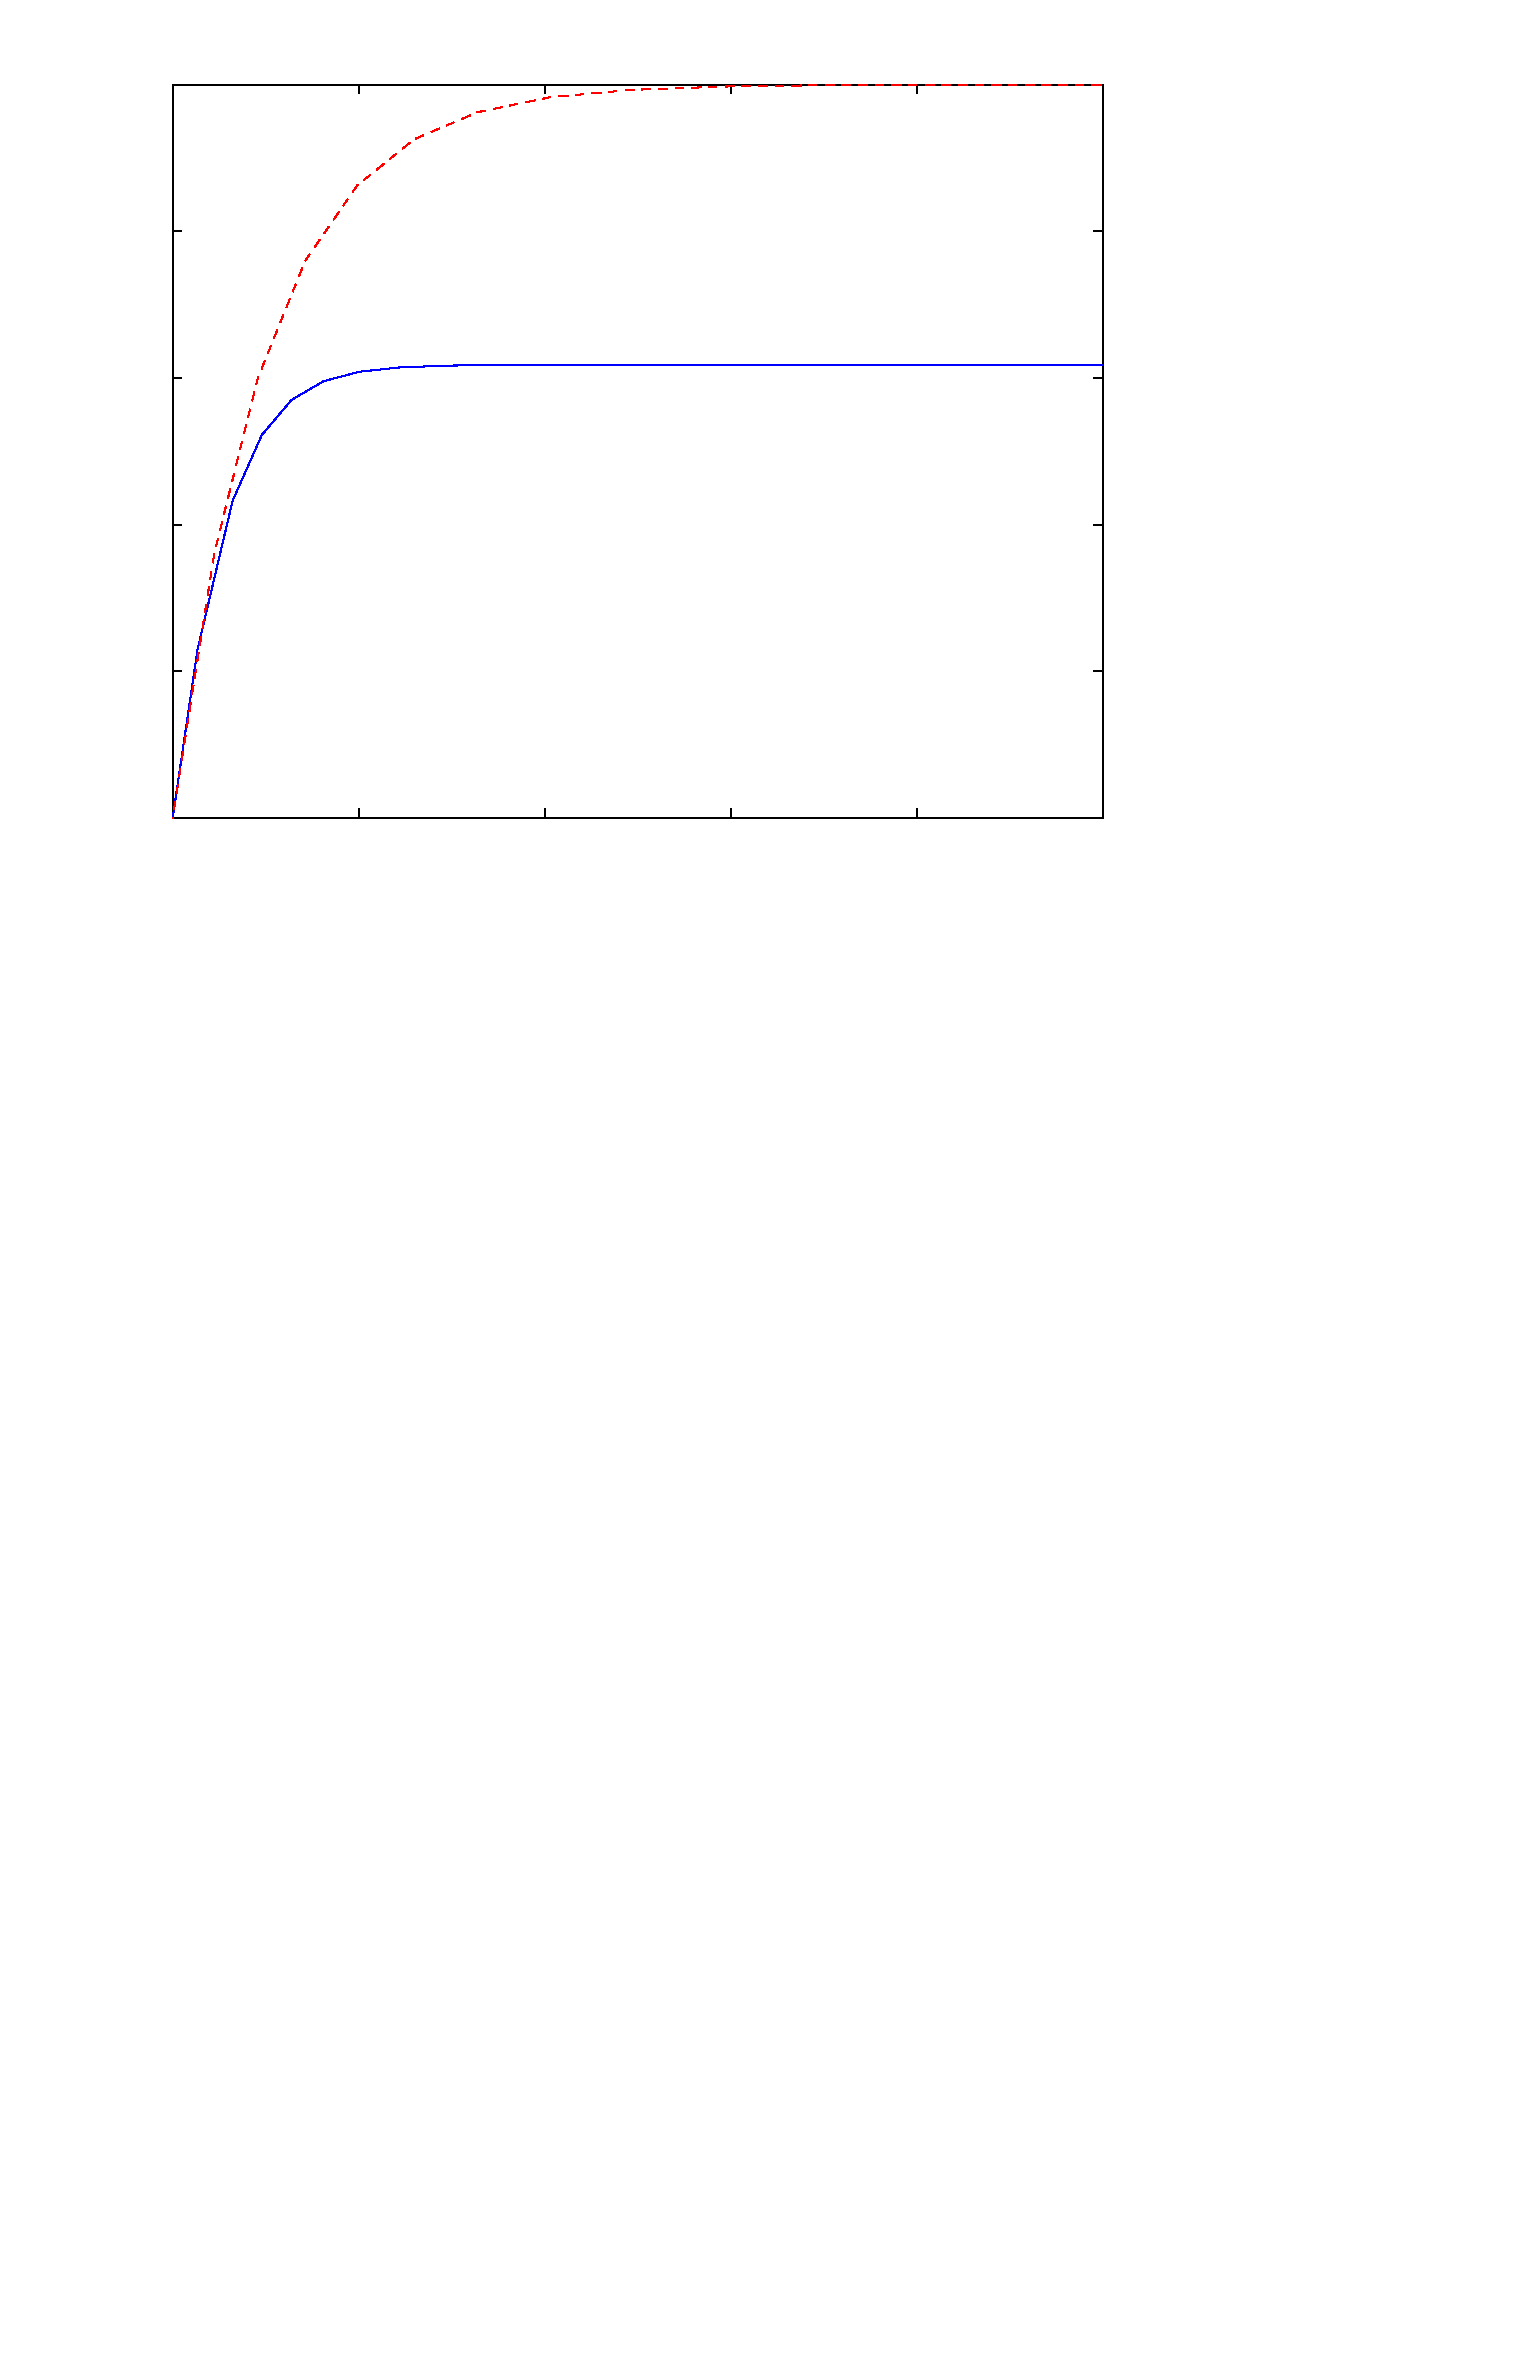
\includegraphics{prog2_fig1-inc}
\end{picture}%
\begin{picture}(717,1119)(0,0)
\fontsize{10}{0}
\selectfont\put(74.88,729.519){\makebox(0,0)[t]{\textcolor[rgb]{0,0,0}{{0}}}}
\fontsize{10}{0}
\selectfont\put(164.16,729.519){\makebox(0,0)[t]{\textcolor[rgb]{0,0,0}{{2000}}}}
\fontsize{10}{0}
\selectfont\put(253.44,729.519){\makebox(0,0)[t]{\textcolor[rgb]{0,0,0}{{4000}}}}
\fontsize{10}{0}
\selectfont\put(342.72,729.519){\makebox(0,0)[t]{\textcolor[rgb]{0,0,0}{{6000}}}}
\fontsize{10}{0}
\selectfont\put(432,729.519){\makebox(0,0)[t]{\textcolor[rgb]{0,0,0}{{8000}}}}
\fontsize{10}{0}
\selectfont\put(521.28,729.519){\makebox(0,0)[t]{\textcolor[rgb]{0,0,0}{{10000}}}}
\fontsize{10}{0}
\selectfont\put(69.8755,734.52){\makebox(0,0)[r]{\textcolor[rgb]{0,0,0}{{0}}}}
\fontsize{10}{0}
\selectfont\put(69.8755,804.936){\makebox(0,0)[r]{\textcolor[rgb]{0,0,0}{{0.002}}}}
\fontsize{10}{0}
\selectfont\put(69.8755,875.352){\makebox(0,0)[r]{\textcolor[rgb]{0,0,0}{{0.004}}}}
\fontsize{10}{0}
\selectfont\put(69.8755,945.768){\makebox(0,0)[r]{\textcolor[rgb]{0,0,0}{{0.006}}}}
\fontsize{10}{0}
\selectfont\put(69.8755,1016.18){\makebox(0,0)[r]{\textcolor[rgb]{0,0,0}{{0.008}}}}
\fontsize{10}{0}
\selectfont\put(69.8755,1086.6){\makebox(0,0)[r]{\textcolor[rgb]{0,0,0}{{0.01}}}}
\fontsize{10}{0}
\selectfont\put(298.08,718.519){\makebox(0,0)[t]{\textcolor[rgb]{0,0,0}{{t}}}}
\fontsize{10}{0}
\selectfont\put(38.8755,910.56){\rotatebox{90}{\makebox(0,0)[b]{\textcolor[rgb]{0,0,0}{{c}}}}}
\fontsize{10}{0}
\selectfont\put(298.08,1096.6){\makebox(0,0)[b]{\textcolor[rgb]{0,0,0}{{Scenario One: Ode 1 (blue,solid), Ode 2 (red,dash)}}}}
\end{picture}
}
    \label{fig:minilab-scenario-one}
  \end{figure}

  \begin{figure}
    \centering
    \caption{Scenario Two}
    \scalebox{0.85}{\huge% Title: glps_renderer figure
% Creator: GL2PS 1.3.9, (C) 1999-2015 C. Geuzaine
% For: Octave
% CreationDate: Mon Feb  8 03:27:48 2016
\setlength{\unitlength}{1pt}
\begin{picture}(0,0)
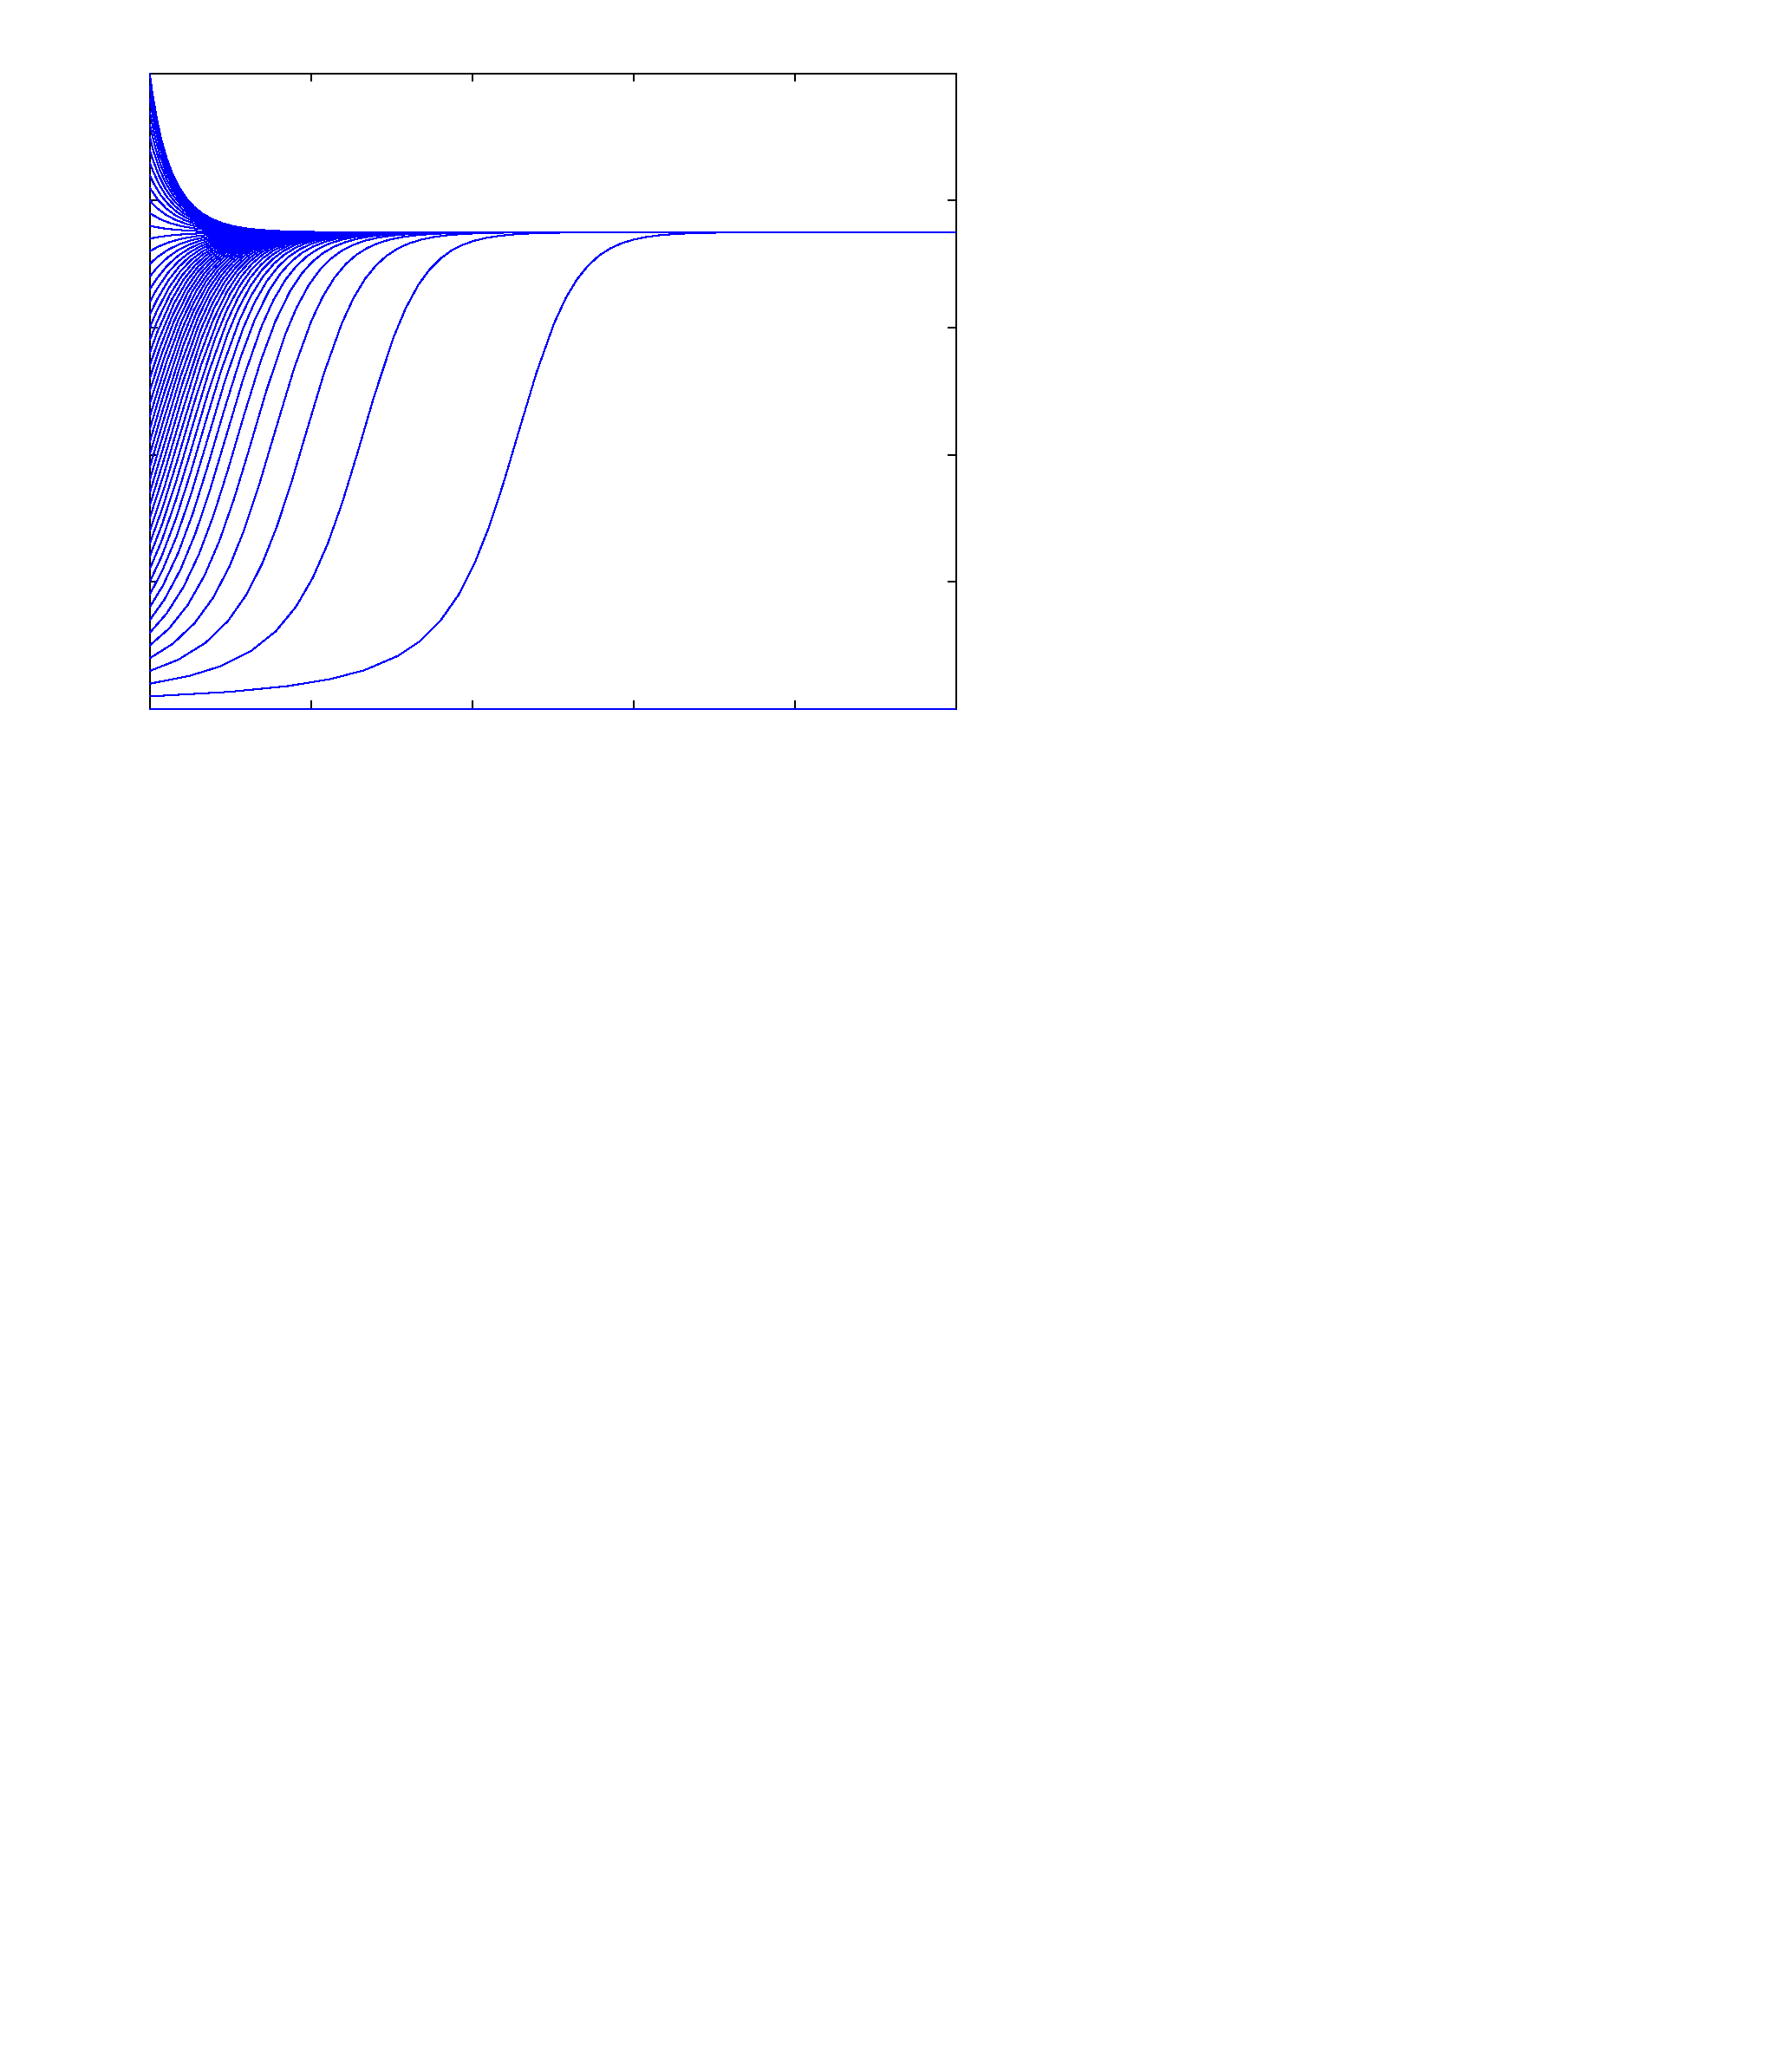
\includegraphics{prog3_fig2-inc}
\end{picture}%
\begin{picture}(717,1119)(0,0)
\fontsize{10}{0}
\selectfont\put(74.88,729.519){\makebox(0,0)[t]{\textcolor[rgb]{0,0,0}{{0}}}}
\fontsize{10}{0}
\selectfont\put(164.16,729.519){\makebox(0,0)[t]{\textcolor[rgb]{0,0,0}{{20}}}}
\fontsize{10}{0}
\selectfont\put(253.44,729.519){\makebox(0,0)[t]{\textcolor[rgb]{0,0,0}{{40}}}}
\fontsize{10}{0}
\selectfont\put(342.72,729.519){\makebox(0,0)[t]{\textcolor[rgb]{0,0,0}{{60}}}}
\fontsize{10}{0}
\selectfont\put(432,729.519){\makebox(0,0)[t]{\textcolor[rgb]{0,0,0}{{80}}}}
\fontsize{10}{0}
\selectfont\put(521.28,729.519){\makebox(0,0)[t]{\textcolor[rgb]{0,0,0}{{100}}}}
\fontsize{10}{0}
\selectfont\put(69.8755,734.52){\makebox(0,0)[r]{\textcolor[rgb]{0,0,0}{{0}}}}
\fontsize{10}{0}
\selectfont\put(69.8755,804.936){\makebox(0,0)[r]{\textcolor[rgb]{0,0,0}{{0.002}}}}
\fontsize{10}{0}
\selectfont\put(69.8755,875.352){\makebox(0,0)[r]{\textcolor[rgb]{0,0,0}{{0.004}}}}
\fontsize{10}{0}
\selectfont\put(69.8755,945.768){\makebox(0,0)[r]{\textcolor[rgb]{0,0,0}{{0.006}}}}
\fontsize{10}{0}
\selectfont\put(69.8755,1016.18){\makebox(0,0)[r]{\textcolor[rgb]{0,0,0}{{0.008}}}}
\fontsize{10}{0}
\selectfont\put(69.8755,1086.6){\makebox(0,0)[r]{\textcolor[rgb]{0,0,0}{{0.01}}}}
\fontsize{10}{0}
\selectfont\put(298.08,718.519){\makebox(0,0)[t]{\textcolor[rgb]{0,0,0}{{t}}}}
\fontsize{10}{0}
\selectfont\put(38.8755,910.56){\rotatebox{90}{\makebox(0,0)[b]{\textcolor[rgb]{0,0,0}{{c}}}}}
\fontsize{10}{0}
\selectfont\put(298.08,1096.6){\makebox(0,0)[b]{\textcolor[rgb]{0,0,0}{{Scenario Two: Ode 1 (blue,solid), Ode 2 (red,dash)}}}}
\end{picture}
}
    \label{fig:minilab-scenario-two}
  \end{figure}

\end{document}
